\subsection{Bitcoin Time Series Data}

- data taken from Blockchain.com API \cite{Data}
- features: classical asset data \& Bitcoin specific data
- in total 3576 days for all the features
- exclude market cap, transaction vol., miner's revenue

\begin{figure}
  \centering
  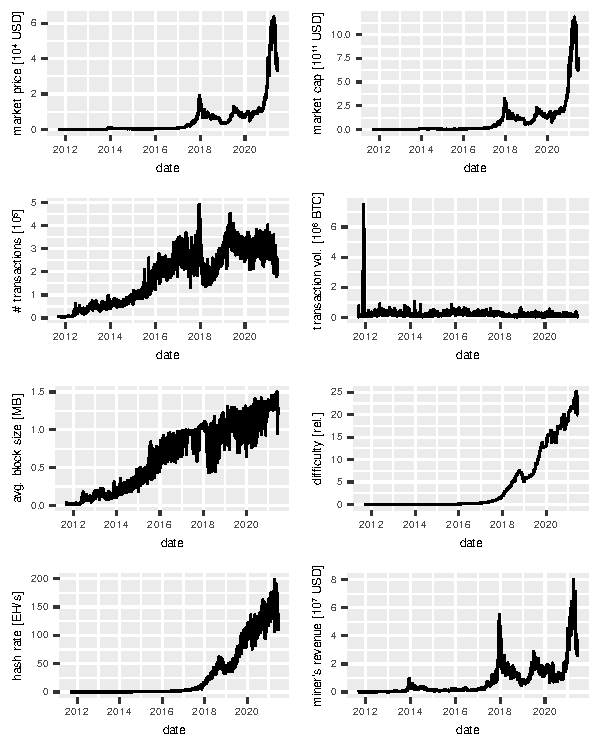
\includegraphics[width=\textwidth]{data.pdf}
  \caption{time series of label and features.}
\end{figure}

\begin{figure}
  \centering
  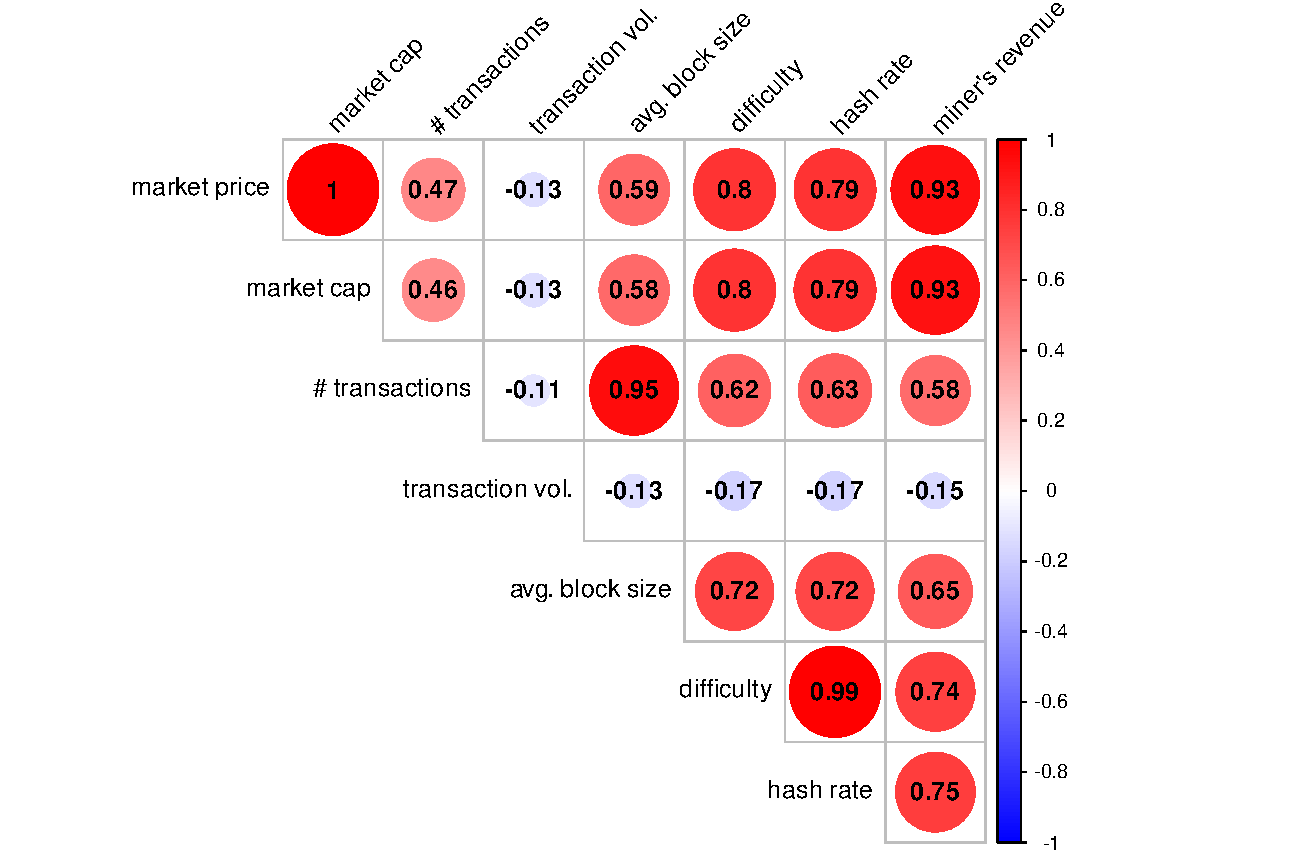
\includegraphics[width=\textwidth]{cor_mat.pdf}
  \caption{correlation matrix with Pearson's correlation coefficient}
\end{figure}

\begin{figure}
	\centering
	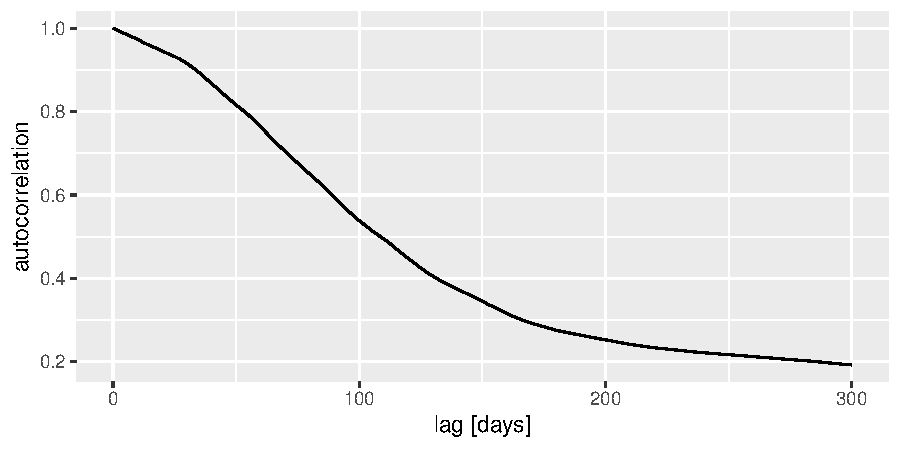
\includegraphics[width=\textwidth]{autocorrelation.pdf}
    \caption{autocorrelation of Bitcoin market price}
\end{figure}

\subsection{Supervised Learning Approach}
- moving window approach with window size $m$ and prediction horizon of $1$
- label 1 if next day sees Bitcoin price increasement, else label 0
- use moving/sliding window technique to transform time series data into labeled supervised learning examples for a classification task
- features are normalized using min-max-method

\begin{figure}
	\centering
	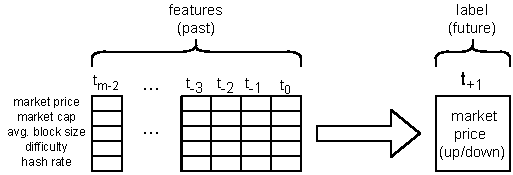
\includegraphics[width=\textwidth]{moving_window.pdf}
    \caption{supervised learning example using moving window technique}
\end{figure}